\documentclass[./00PhotoBox.tex]{subfiles}
\graphicspath{{\subfix{./img/}}}
\begin{document}


\chapter{Voruntersuchungen}
Vor und während des Aufbaues des eigendlichen Messystemes wurden einige Voruntersuchungen durchgeführt. Diese dienten dazu, die Machbarkeit des Systemes zu prüfen und die notwendigen Schritte zu ermitteln und zu optimieren.


\section{Änderung der Kamerakonstante durch Fokussierung}

\paragraph{These}
Die Kamerakonstante einer Kamera ändert sich durch die Fokussierung. Bei gleich eingestellter Objektdistanz ist die Kamerakonstante näherungsweise gleich sein.

\paragraph{Ziel}
In \citet[S. 146]{luhmann} wird eine Näherungsformel (siehe \autoref{eq:luhmann_fokus}) für die \Gls{Kamerakonstante} in Abhängigkeit des Fokus gegeben. Diese soll überprüft werden und eine optimierte Formel für die Raspberry Pi Kamera ermittelt werden.

\begin{align}
    \frac{1}{f} = \frac{1}{c} + \frac{1}{d}
    \label{eq:luhmann_fokus}
\end{align}

\paragraph{Vorgehen}
Die Änderungen wurden in einem Versuch beobachtet. Hierzu wurde der Raspberry Pi Zero mit montierter Kamera fest vor einem Charuco-Kalibriermuster platziert. Dieser ermöglicht auch bei unscharfen Bildern noch eine gute automatische Erkennung der zu beobachtenden Punkte. Es wurden je 11 Bilder mit unterschiedlichen Fokussierungen von $2~\text{m}$ bis  $10~\text{cm}$ aufgenommen. Dieser Vorgang wurde insgesamt viermal wiederholt, um auch die Wiederholungsgenauigkeit zu ermitteln. Die Bilder wurden anschließend mit einem Python-Script unter Nutzung von OpenCV ausgewertet. Hierbei wurde die relative Veränderung der Kamerakonstante der Kamera ermittelt und mit dem erwarteten Wert verglichen.

\paragraph{Ergebnis}


\begin{figure}
    \centering
    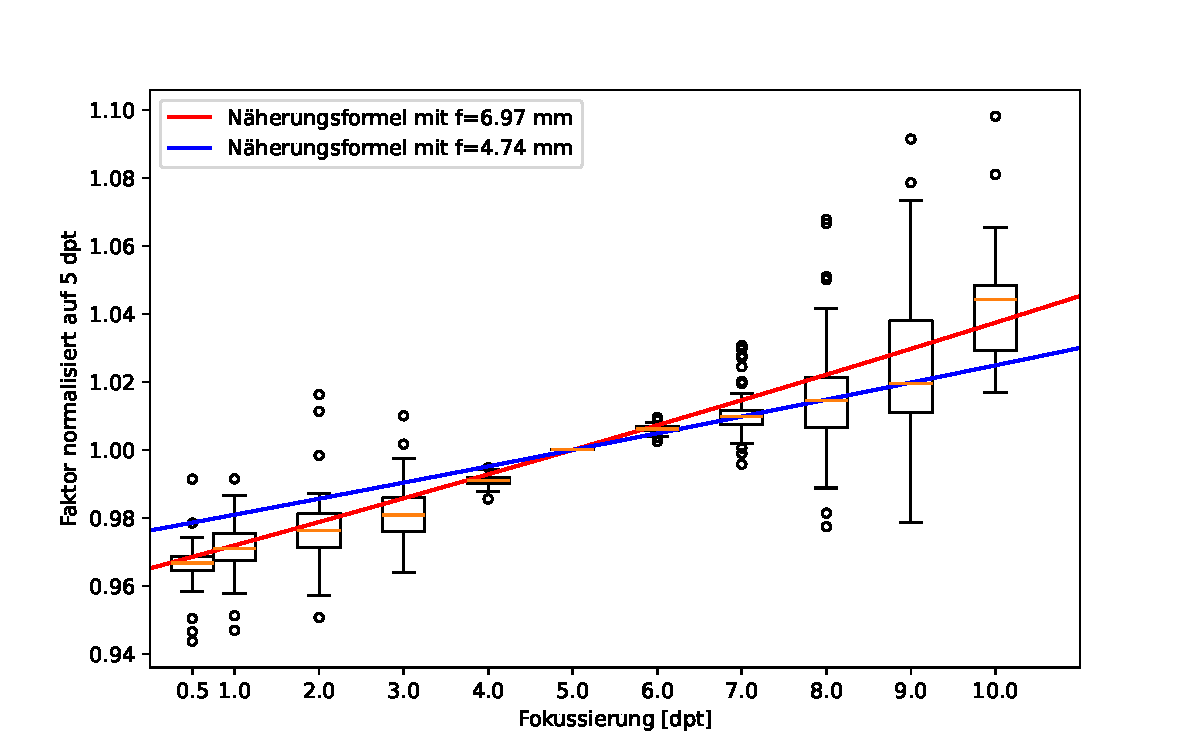
\includegraphics[width=1\textwidth]{./img/fokus_faktor_diagramm_box.pdf}
    \centering
    \caption{Box-Whisker-Plot der relativen Veränderung der Kamerakonstante normalisiert auf eine Fokusdistanz von 20 cm (5 dpt)} %Bildunterschrift
    \label{img:fokus_faktor} %ID fürs Bild
\end{figure}



\section{Änderung der Verzeichnung}

\paragraph{These}
Durch die Verschiebung der Linsen verändert sich auch die Verzeichnung der Kamera.

\paragraph{Ziel}
Die Veränderung der Verzeichnung soll ermittelt und eine Korrekturformel ermittelt werden.

\paragraph{Vorgehen}

\begin{itemize}
    \item Kamera fest positioniert (keine Änderungen durch Schwerkraft)
    \item jeweils festen Fokus
    \item ChAruco-Board wird bewegt
\end{itemize}

\section{3D-Modell aus Fokusstacking}

\paragraph{These}
Durch Fokusstacking kann ein besseres 3D-Modell erstellt werden.

\paragraph{Ziel}
Es soll geprüft werden, ob durch Fokusstacking die Qualität des 3D-Modell verbessert werden kann. Hierzu wird ein 3D-Modell aus einem Fokusstacking erstellt und mit einem normalen 3D-Modell verglichen.

\paragraph{Vorgehen}
\begin{itemize}
    \item Automatisierter Fokusstacking
    \item keine Beachtung der festen Ausrichtung
    \item Transformation über SIRF und Homographie
\end{itemize}

\biblio
\end{document}